\documentclass[a4paper]{article}
\usepackage{float}
  
\usepackage[spanish]{babel}
\usepackage[utf8x]{inputenc}
  
\usepackage[spanish]{babel}
\usepackage[utf8x]{inputenc}
\usepackage{amsmath}
\usepackage{graphicx}
\usepackage[colorinlistoftodos]{todonotes}

\date{\today}
\author{Alejandra Gpe. Esquivel Guillén \\ alejandraeg9899@gmail.com}
\title{Sistemas de Recomendación}

\begin{document}
\maketitle

\section{Objetivos}
Este trabajo busca esbozar las características de un sistema de recomendación, su impacto en los negocios modernos. Resaltar los algoritmos que se utilizan en su diseño. Mostraremos cómo estos sistemas obtienen las preferencias de los usuarios y presentaremos un caso de estudio donde usamos el algoritmo de vecinos cercanos. 

Los sistemas de recomendación(SR) son componentes cruciales para los negocios en linea, con ellos se busca mantener a sus usuarios satisfechos e incrementar el número de ventas diarias por usuario. Por ello considero que el conocimiento de estos sistemas, son una de las tendencias más importantes de la computación de nuestro tiempo.

\section{Introducción}
Los SR aparecen a mediados los 80 de manera natural, por los vendedores que buscaban entender lo que sus clientes deseaban comprar, se generaban catálogos impresos y se entregaban con cupones dentro, en los hogares de los clientes. Con la entrada del internet y el auge del correo electrónico se inició el acercamiento usando listas de correo, muy pronto se vio la necesidad de sumar clientes o visitas de ellos al sitio web corporativo del negocio para dar variedad al catálogo. Gracias a los avances en los algoritmos de minería de datos se observó que algunas herramientas estadísticas podían usarse para anticiparse a las preferencias si conocíamos el perfil de otros usuarios con características similares. Fue así que iniciaron como simple observación de las preferencias de los
clientes y en un inicio sólo  se ofrecían listas de los artículos más comprados por otros usuarios de temporada. Con frecuencia los individuos confiaban en las
recomendaciones ofrecidas por otros; de la misma manera que alguien
te recomienda un libro o una película. La escala de evaluación comenzó
en la mayoría de los productos con una escala fija (A = bueno, B =
regular, C = malo) en donde se establece el valor de cierta variable
(calidad, precio, disponibilidad).
Los sistemas de recomendación hoy en día juegan un rol importante en todos los sitios web. La meta de ellos
es incrementar las ventas, visitas, variedad de contenidos y presentar experiencias de usuario
personalizadas ofreciendo sugerencias para artículos desconocidos
potencialmente interesantes para un usuario.

Los SR actuales utlizan algoritmos avanzados y se invierten grandes recuersos en su desarrollo.

El interés en esta área permanece alto debido a que constituye un
problema rico en investigación y a la abundancia de aplicaciones
prácticas que ayuden a los usuarios a lidiar con sobrecarga de
información.

Las grandes compañías de medios fueron las primeras en invertir en
SR. En 2006 Netflix lanzó una competencia para mejorar su entoces sistema de recomendación en al menos un 10\% de efectividad.

El rol clave de los sistemas de recomendación es que se basan en mineria de datos, rama de la computación que se encuentra en auge y que utiliza algoritmos de inteligencia artificial obteniendo conocimiento a partir de la información.

Sin embargo, a pesar de todos estos avances, la actual generación de
sistemas de recomendación evolucioana rapidamente presentando retos imposibles de resolver por la arquitectura computacional requerida como consecuencia esto a llevado a una competencia entre las empresas por vender la 'mejor solución'. Lo que se busca al diseñar un SR es que se adapte a la inmensa cantidad de información generada por los usuarios optimizando la memoria requerida. Los SR se aplican a un rango amplio de casos como
recomendaciones vacacionales, ciertos tipos de servicios bancarios o de
financiamiento a inversionistas, y productos a ser vendidos en una
tienda creada por un 'carrito inteligente'. Estas mejoras
incluyen mejores métodos para representar comportamiento y la
información acerca de los artículos ha ser adquiridos, métodos avanzados
de recomendación, incorporación de información contextual y utilización
de ratings multicriterio, además del desarrollo de métodos menos
intrusivos que también se apoyan en métricas para determinar desempeño
de los sistemas de recomendación.

\begin{itemize}

\item La recolección de preferencias de los usuarios: \textbf{ No
tiene nada que ver con los perfiles de usuario} ya que esto se realiza a
través de una encuesta que permite conocer las preferencias de los
usuarios, algunos de ellos mencionan las características deseables de un
artículo específico.

\item Análisis: \textbf{ En esta etapa se detectan
patrones en las opciones seleccionadas por los usuarios. - }
\item Generación de opciones:  Los SR se modifican continuamente debido a que el
usuario interacciona con el catalogo de artículos y el SR debe adaptarse
dinámicamente a dichos cambios.

\item Artículos Recomendados: Los
artículos pueden ser en general cualquier bien o servicio requerido por
un usuario específico. No se requiere que el usuario tenga experiencia
previa con el uso del sistema principal. Sin embargo sus selecciones son
tomadas en cuenta para mejorar la precisión de la recomendación próxima.

\end{itemize}

\subsection{Carácteristicas clave que un  SR debería cumplir}

\begin{itemize}
\item
  \textbf{Incrementar el número de artículos vendidos}: Debería ser capaz
  de vender un conjunto de artículos de modo que puedan ser comprados
  sin la intervención de los SR, es decir puede tener su propia meta de
  venta (** ningún visitante se puede ir sin comprar **).
\item
  \textbf{Vender artículos diversos}: Se prefiere la diversidad de
  artículos al ofertar productos ya que las empresas buscan que los
  usuarios (clientes) detecten productos en los que ni siquiera han
  pensado adquirir. Con frecuencia se dan descuentos o rebajas en ellos
  lo que ocasiona que las recomendaciones de los usuarios impacten su
  venta.
\item
  \textbf{Incrementar la satisfacción del usuario}: Un SR bien diseñado
  cambia la interfaz de usuario según las preferencias de los mejores
  clientes, ofreciendo objetivos resaltados y posibilidad de que en base
  a los cambios de la interfase se crean grupos de interés para ofertar
  productos.
\item
  \textbf{Mejor entendimiento de lo que el usuario quiere}: El sondeo
  adecuado de las preferencias del usuario, permite afinar los
  parámetros del SR con el fin de acertar en el ``mejor'' producto.
\item
  \textbf{Incrementar la fidelidad del usuario}: La interacción por
  parte del usuario con el sitio permite que la información sea dinámica
  (contenido que mantenga la atención) con frecuencias las sugerencias y
  reseñas de un producto mantienen al usuario mas tiempo en el sitio lo
  que se aprovecha dando mas opciones de compra.
\end{itemize}

\subsection{Clasificación de los SR}

Los SR usualmente son clasificados en las siguientes categorías:

\begin{itemize}

\item
  \textbf{Recomendaciones Basadas en contenido}: Al usuario le serían
  recomendados artículos similares a los que selecciona en el pasado.
\item
  \textbf{Recomendaciones Colaborativas}: Al usuario le serían
  recomendados artículos que gustan a las personas con preferencias y
  gustos similares en el pasado.
\item
  \textbf{Aproximación Híbrida}: Estos métodos combinan métodos
  colaborativos y basados en contenido.
\end{itemize}

Adicionalmente los sistemas de recomendación que predicen valores
absolutos de rating que usuarios individualmente no han marcado aun en
artículos no conocidos, se les conoce como \emph{filtrado basado en
preferencias }.
\section{Importancia de los SR}

El interés  de las empresas y universidades en los SR se basa en que constituye un
problema rico en investigación,  debido la abundancia de aplicaciones
prácticas que ayuden a los usuarios a lidiar con la sobrecarga de
información; y además el beneficio económico que se puede obtener de ellas.

Las grandes compañías de medios fueron las primeras en invertir en
máquinas de aprendizaje comerciales. En 2006, Netflix anunció su máquina
de aprendizaje y la competencia de minería de datos Netflix Prize con 1 millón de
dólares para el equipo que logrará mejorar su entonces recomendador, el cual fue reclamado en 2009, con toda la atención de
los medios, lo que se conoció como `Recomendaciones de Netflix: Más allá
de las 5 estrellas', reveló  que la ciencia de los datos (Science Data) puede ser una grán inversión para cualquier negocio en linea y que las ciencias de la computación en la rama de aprendizaje automático tienen algoritmos que pueden ser adaptados a sistemas comerciales. La meta de Netflix Prize
fue fondear un algoritmo de recomendaciones que pudiera entregar 10\% de
mejora en precisión de predicción sobre el sistema existente para ello utilizaron herramientas conocidas como Deep Learning. Apple basa
su sistema de recomendaciones de estrenos en el sistema de crítica
Rotten Tomatoes. Google Play Store en un sistema de ranking de
aplicaciones.

Sin embargo, a pesar de todos estos avances, la actual generación de
sistemas de recomendación aún requieren mejoras para realizar métodos
más efectivos y que sean aplicables a un rango amplio de casos, tales como
recomendaciones vacacionales, servicios bancarios o de
financiamiento a inversionistas, y productos a ser vendidos en una
tienda creada por un ``carrito inteligente''. 
Estas mejoras
incluyen  métodos para representar el comportamiento  de los usuarios y la
información acerca de los artículos que van a ser adquiridos; métodos avanzados
de recomendación; incorporación de información contextual (Ubicación Geográfica, Usuarios satisfechos del producto, etc) y utilización
de ratings multicriterio. Además se deben desarrollar métodos no
intrusivos que también se apoyan en métricas para determinar desempeño
de los sistemas de recomendación.

\section{Antecedentes}

Las raíces de los sistemas de recomendación inician con trabajos en
ciencia cognitiva, recuperación de información y algunas conexiones con
administración científica, emergen como un área independiente a mediados
de 1990 cuando los investigadores se enfocan en problemas de
recomendación que explícitamente se basaban en una estructura de rating.
Intuitivamente, esta estimación es usualmente basada en la escala
definida por un usuario acerca de una breve información. A partir del
rating de algunos artículos se puede determinar el rating de algunos que
no han sido seleccionados, con el \textbf{rating superior estimado} . De
manera formal el problema de recomendación puede ser formulado como
sigue: Sea $C$ el conjunto de todos los usuarios y sea $S$ el
conjunto de los posibles artículos que pueden ser recomendados tales
como libros, películas o restaurantes. El espacio $S$ de los posibles
artículos puede ser muy amplio, alcanzando los cientos de millones de
artículos. Similarmente el espacio del usuario puede ser bastante
amplio. Sea $u$ la función de utilidad que mide el beneficio de un
articulo $s$ al usuario. De modo que $C \times S \rightarrow R$,
donde $R$ es la totalidad de un conjunto ordenado. Entonces, para cada
usuario $c \in C$, queremos seleccionar tal $s' \in S $ que
maximiza la utilidad del usuario. De manera simplificada tenemos que:
$\forall c \in C, s'=arg max u(c,s)$

En un sistema de recomendación la utilidad de un artículo es usualmente
representada por un \emph{rating} el cual indica como a un usuario le gusta un artículo en particular. Por ejemplo: Juan Perez le dio a
``Harry Potter'' el rating de 7 (en escala de 1 a 10).

\textbf{Ratings}. Rotten Tomatoes (Tomatómetro): El rating del
tomatómetro se basa en las opciones publicadas por críticos de cine y
televisión, es una medida confiable de la calidad de una película y
representa el porcentaje de reseñas positivas dadas a una película.

\textbf{Filtrado Colaborativo}: La idea detrás del filtrado colaborativo
es que se pueden usar los rating de los usuarios que comparten gustos
similares para predecir los que aún no han sido definidos. Para obtener
intuición, se comparan los ratings por pares del usuario

\subsection{ Ejemplos de SR:}

\begin{itemize}

\item Airbnb. Sitio de recomendación de hospedaje. 
Promueve el hospedaje en casas o departamentos de particulares que ofrecen habitaciones a bajo precio donde además de mostrar ubicaciones disponibles por fecha y ubicación preferida, se incluye información de reseñas de clientes previos y se mezclan con comentarios de redes sociales relacionadas al perfil del usuario.

\item Yelp. Recomendación de restaurantes. 
Los usuarios publican reseñas de sitios como: Restaurantes, Tiendas, Servicios (Taxi, Tintoreria, Lavanderia) y van construyendo confianza en los proveedores o vendedores de cierto bien, después se publican en un portal donde se localizan ubicandolos por ubicación cercana al cliente.

\item Los SR de grandes empresas como
Google Play, Apple Movies  utilizan un sistema de ranking para sugerir aplicaciones. Un sistema de ranking puede utilizar elementos como el número de descargas, el tamaño de la aplicación, y la ubicación geográfica del vendedor para mostrar en primer lugar las aplicaciones que tienen la misma categoría y que han sido seleccionadas por otros usuarios en compras previas. De manera similar al ranking de las busquedas de google, se cuentan las palabras clave (keywords) y el numero de links a un sitio específico. De ahi que sólo se muestran los primeros 10 sitios más visitados. 
\end{itemize}

\section{Descripción del Problema}\label{descripciuxf3n-del-problema}

Se consideraá una empresa dedicada a la venta y renta de inmuebles cuyos canales  de venta són  entrevistas y mediante llamadas telefónicas. Ha decidido invertir en un sitio web donde publica el listado de propiedades a ofertar. Como en la mayoria de sitios web el diseño se centra unicamente en ser un portal informativo y poca interacción con el usuario. Por consecuencia los clientes que visitan el sitio (ver info de visitas) observan que resulta muy complicado localizar alguna propiedad relevante. O las que se muestran como relevantes están fuera de su presupuesto.

Este ejemplo es el caso de la mayoria de negocios mexicanos que utilizan un portal web para anunciarse y no aprovechan la interacción con sus clientes.
Dentro de la ciudad de Morelia, se han detectado poco más de 30 inmobiliarias que utilizan portales para promoción, incluso las principales constructoras (Arko, Habicasa) utilizan  portales de tipo informativo. Este proyecto busca incrementar la cantidad de información que un usuario promedio recibe al consultar una propiedad incluyendo opciones similares con el fin de mantener el usuario más tiempo en sitio y por consecuencia incrementar la utilidad de la información. Durante la navegación se buscará conocer al usuario a través de breves cuestionarios sobre la información que se está consultando para identificar potenciales opciones. 

\subsection{Metodología}

Nuestra propuesta de diseño se centra en 4 puntos.
\begin{enumerate}
\item Crear un Marco de Datos, recopilando información de inmobiliarias de la ciudad de Morelia.
\item Identificar usuarios potenciales que deseen adquirir propiedades.
\item Proporcionar sugerencias cercanas a las deseadas.
\item Medir la precisión a través de encuestas de satisfacción al cliente.
\end{enumerate}


\subsection{Recolección de los datos}

Para la recolección se  utilizo un crawler publico{[}6{]} que indexa las paginas web de las inmobiliarias, de ahí obtenemos una lista de links (ver figura 1), filtramos la lista dejando unicamente las que se refieren a propiedades y almacenanos los documentos en HTML. Extraemos el corpus con python y almacenamos cada propiedad en el dataset para convertirlo a un archivo csv con el cual realizaremos la clasificación de las propiedades.
\begin{figure}[h]
\centering
\begin{tabular}{cc}
  \hline
 & Total \\ 
  \hline
Bodega &   5 \\ 
  Casa & 168 \\ 
  Departamento &  24 \\ 
  Edificio &   1 \\ 
  Local &  13 \\ 
  Oficinas &   1 \\ 
  Terreno &  72 \\ 
   \hline
\end{tabular}
\caption{Tabla de Propiedades por Inmueble}
\end{figure}


\begin{figure}[htbp]
\centering
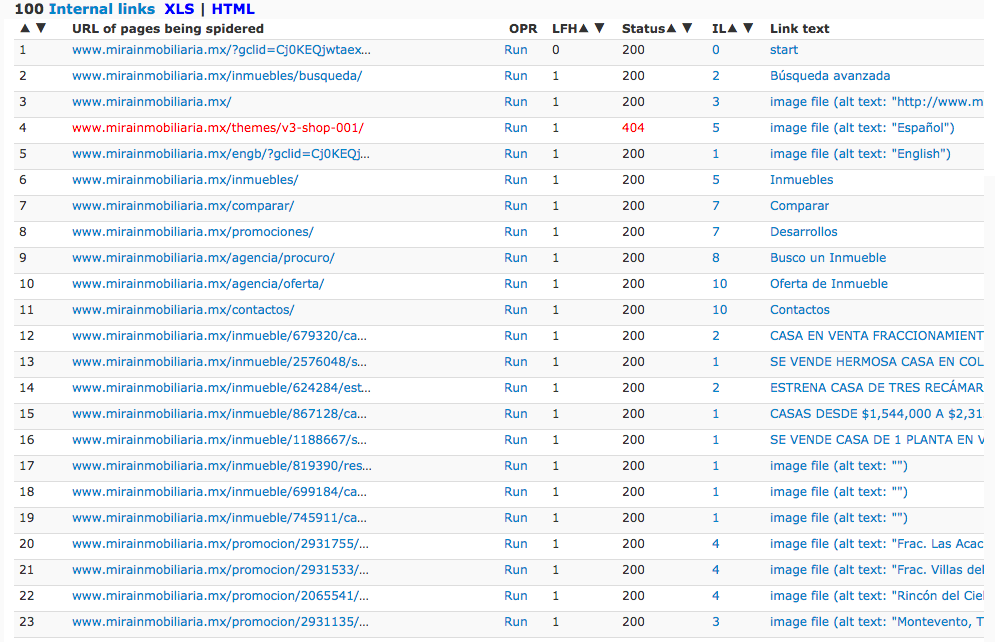
\includegraphics[width=0.8\textwidth]{CrawlerSite.png}
\caption{Listado de Artículos relacionados con propiedades}
\end{figure}

\begin{figure}[htbp]
\centering
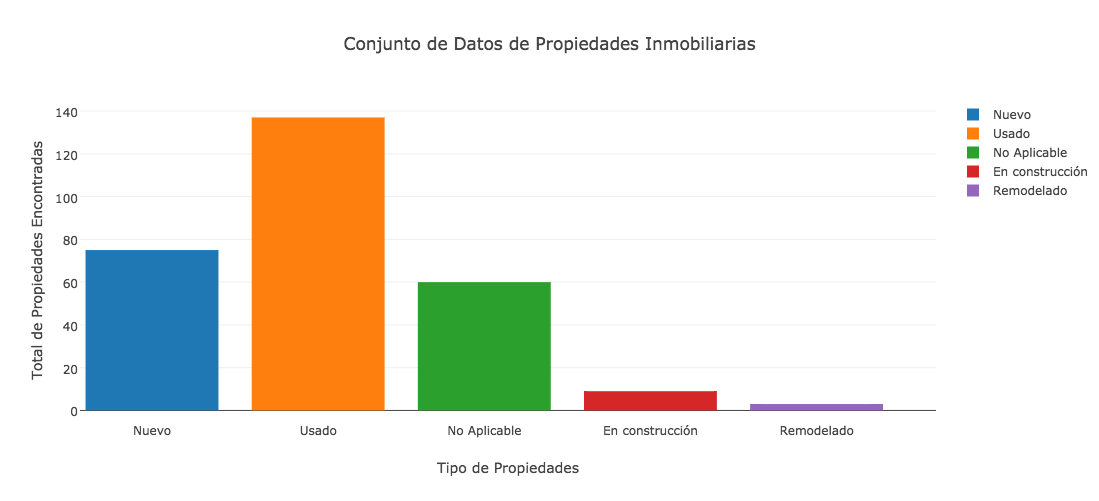
\includegraphics[width=0.8\textwidth]{PropiedadesInmobiliariasEstadoVivienda.png}
\caption{Distribución de Propiedades Tipo de Propiedad}
\end{figure}

\subsection{Clasificación de las propiedades}
Para el procesamiento de los datos decidimos utilizar el lenguaje de programación R, para analizar y clasificar. Las propiedades que descargamos de los web sites las hemos agrupado en un solo listado con aproximadamente 500 propiedades, las cuales  vienen listadas por Estado (Usado, Nuevo, Construcción), Área construida ($m^2$), Zona (Colonia o barrio de Referencia), Precio, Latitud, Longitud y algunas otras características deseadas.  El algoritmo de clasificación para esta sección que hemos seleccionado es el de vecinos cercanos ya que estamos trabajando con variables categóricas, nuestro objetivo es analizar si podemos definir clases de propiedades.
\begin{figure}[htbp]
\centering
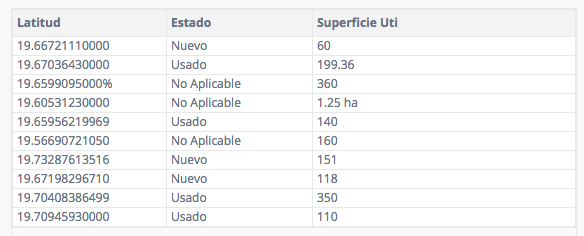
\includegraphics[width=0.8\textwidth]{Dataset.png}
\caption{Dataset de Propiedades Inmobiliarias}
\end{figure}


\subsection{KNN - Nearest Neighbor}
También conocido como K-nearest Neighbor es el más simple de los algoritmos de aprendizaje máquina que existe y el más utilizado. Se basa en identificar los k  registros en el conjunto de entrenamiento que son "cercanos" en similaridad. La prueba asigna una clase a la mayoria de los vecinos cercanos. El K-NN trata las caracteristicas como coordenadas multidimensionales. Para ejemplo tomamos las características de un conjunto de prueba que definimos como ingredientes. El algoritmo requiere un conjunto entrenamiento y un conjunto prueba, en nuestro caso usamos para entrenamiento únicamente las casas con estado = 'usado'.

\subsection{Metrica de similaridad con distancia.}

El Knn requiere una función distancia, o una fórmula que mida la similaridad entre dos instancias. Existen diferentes maneras de calcular la distancia. Tridicionalmente el Knn utiliza la distancia euclideana, que es la distancia de un punto con respecto a otro conectados por una linea o regla. La distancia euclideana se expresa de la siguiente manera:
\begin{equation}
dist(x,y) = \sqrt{(p_1-q_1)^2 + (p_2-q_2)^2+ \cdots + (p_n - q_n)^2}
\end{equation}

La desición de cuantos vecinos cernanos para el uso de K-NN determina que tan bien el modelo generaliza para futuros datos. El balance entre sobre ajustar o subajustar el conjunto de entrenamiento es un problema conocido como Ajuste de la varianza. Seleccionando valores de K reduce el impacto de la varianza causada por datos ruidosos, pero puede que el sistema ignore los grupos pequeños, pero importante patrones. En el lado opuesto usando una k mayor se influye sobre la muestra clasificada. Obviamente, el mejor valor de k se encuentra entre estos dos extremos.
\begin{figure}[h]
\centering
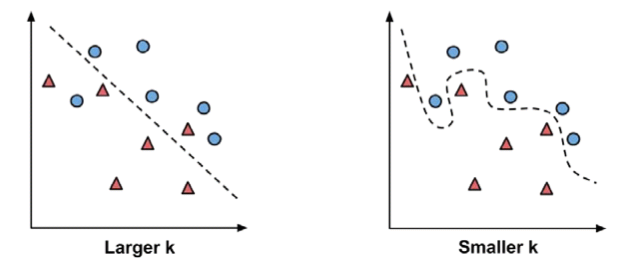
\includegraphics[width=0.5\textwidth]{IMG_0061.png}
\caption{Selección de la k en KNN}
\end{figure}






\section{Resultados}
De la figura 4 podemos analizar que de una entrada dada de 40 selecciones se puede sugerir un conjunto de propiedades con una K de 7 probamos distintos valores de K para refinar la consulta y obtener resultados con características similares a la entrada de datos.
Sin embargo al utilizaar este algoritmo utilizamos una función de normalización de los datos buscando que las propiedades consideradas en la misma escala, se afecta el resultado del clasificador.


\begin{figure}[h]
\centering
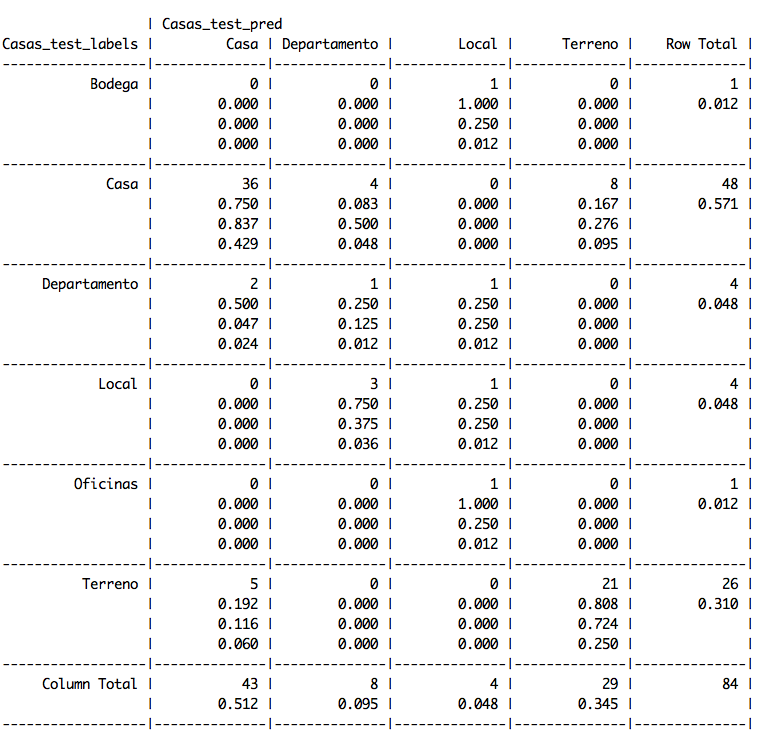
\includegraphics[width=0.9\textwidth]{ModeloPredictivo.png}
\caption{Propiedades recomendadas según la selección del Usuario}
\end{figure}
\section{Bibliografía}
{[}1{]}  Adomavicius, G., and A. Tuzhilin. “Toward the next Generation of Re-
commender Systems: A Survey of the State-of-the-art and Possible Extensions.”

IEEE Trans. Knowl. Data Eng. IEEE Transactions on Knowledge and Data En-
gineering: 734-49. Print.

{[}2{]} Sauter, Vicki Lynn, and Vicki Lynn Sauter. Decision Support Systems

for Business Intelligence. 2nd ed. Hoboken, N.J.: Wiley, 2010. Print.

{[}3{]}  R.Bell, Y. Koren and C. Volinsky. The BellKor 2008 Solution to the

Netflix Prize. 2008

{[}4{]} Said, Alan, Brijnesh J. Jain, Sascha Narr, and Till Plumbaum. “Users and
Noise: The Magic Barrier of Recommender Systems.” User Modeling, Adapta-
tion, and Personalization Lecture Notes in Computer Science: 237-48. Print

{[}5{]}  Lantz, B. (n.d.). Machine learning with R: Learn how to use R to apply powerful machine learning methods and gain an insight into real-world applications.

{[}6{]} Harrington, P. (2012). Machine learning in action. Shelter Island, NY: Manning Publications.

{[}7{]} Toomey, D. (n.d.). R for data science.

{[}8{]} Teutonico, D. (2015). Ggplot2 essentials explore the full range of ggplot2 plotting capabilities to create meaningful and spectacular graphs. Birmingham, England: Packt Publishing.

{[}9{]}  Leipzig, J., \& Li, X. (2009). Data mashups in R. Sebastopol, Calif.: O'Reilly.

{[}10{]} Ricci, F. (2011). Recommender systems handbook. New York: Springer.

{[}11{]}  Russell, S., \& Norvig, P. (1995). Artificial intelligence: A modern approach. Englewood Cliffs, N.J.: Prentice Hall.

{[}12{]} Website Crawler Tool and Google Sitemap Generator \\
http://freetools.webmasterworld.com/tools/crawler-google-sitemap-generator/

\end{document}
